\documentclass{article}
\usepackage{amsfonts, amsmath, amssymb, amsthm, dsfont, mathtools, stmaryrd}
\usepackage{enumitem}
\usepackage{graphicx}
\usepackage{setspace}
\usepackage{indentfirst}
\usepackage[margin=1in]{geometry}
\graphicspath{{./images/}}
\setstretch{1.15}
\newtheorem{theorem}{Theorem}
\newtheorem{definition}{Definition}
\newtheorem{lemma}{Lemma}
\newcommand*{\R}{\mathbb{R}} 
\newcommand*{\N}{\mathbb{N}}
\newcommand*{\Z}{\mathbb{Z}}
\newcommand*{\M}{\mathcal{M}}

\title{Trails of Lost Pennies: A Lower Bound to the Mina Margin}
\author{Neo Lee}
\date{November 2023}

\begin{document}

\maketitle

\section{\centering Abstract}
This paper proves a lower bound of $\lambda \geq 0.999902$ to $\lambda =
\inf\{\M(x):x\in0,\infty\}$, which gives a sufficient and necessary condition for the existence of
time-invariant Nash equilibrium in Trails of Lost Pennies.


\section{\centering Introduction / Game Setup}
The Trail of Lost Pennies is a two-player strategic game played on the integer line introduced by
[Hammond]. Below, we will first introduce the finite Trail of Lost Pennies, then its infinite
counterpart. We will eventually prove our results in the infinite game through an approximation to
the finite game.

\subsection{\centering Finite Trail of Lost Pennies}
\begin{figure}[htb!]
    \centering
    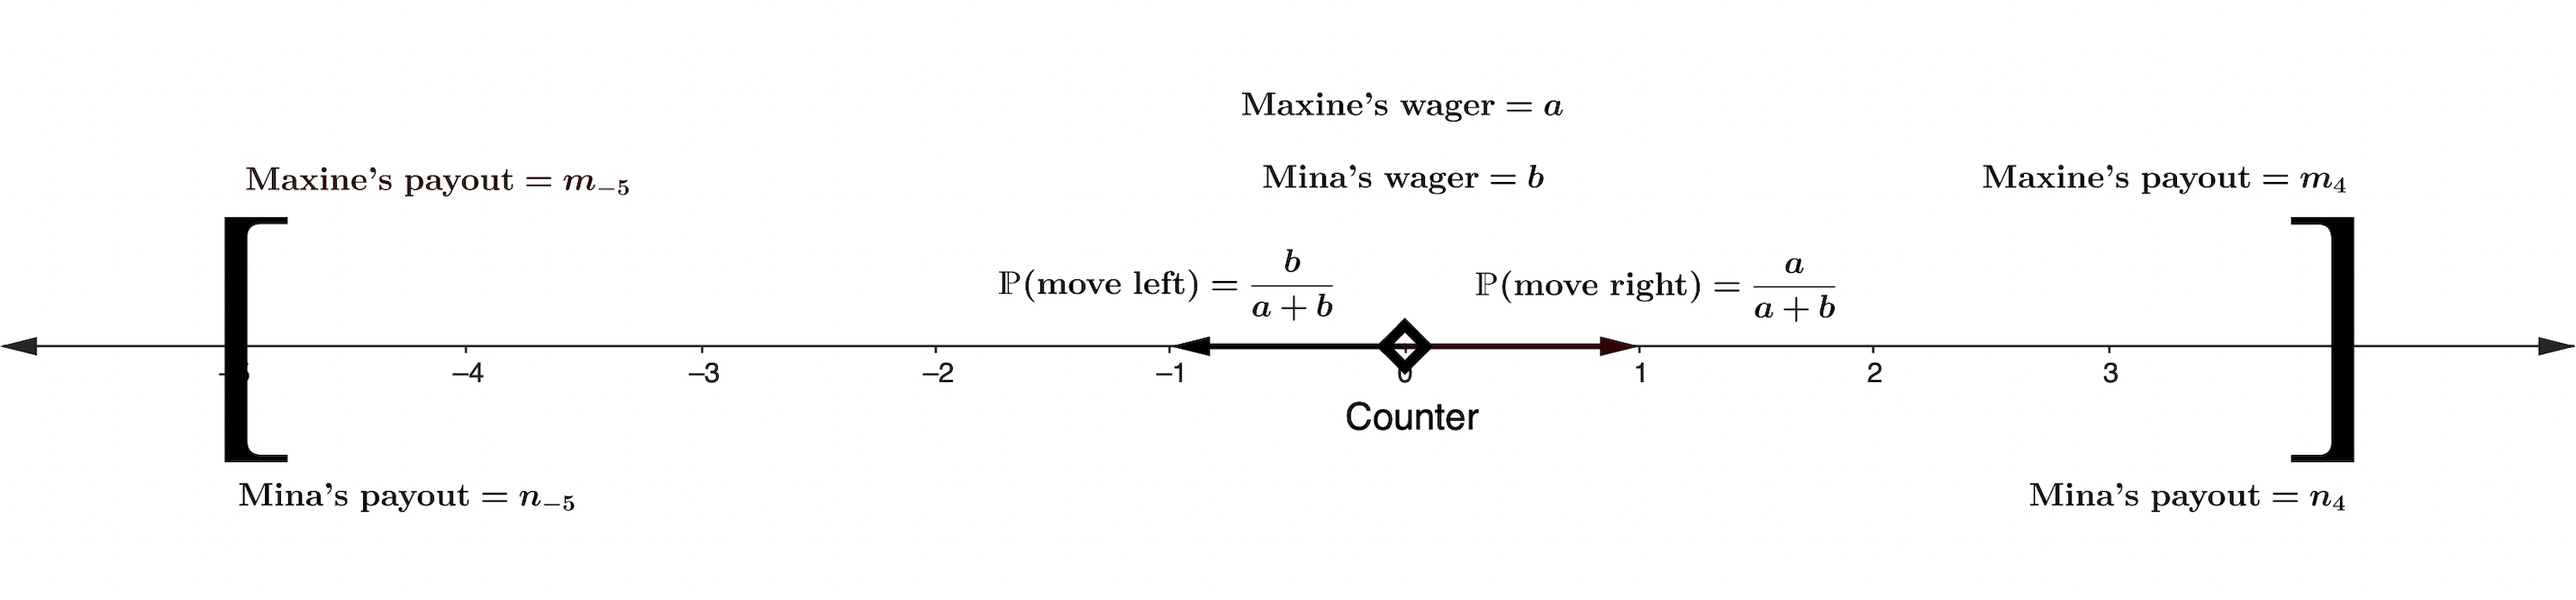
\includegraphics[scale=0.3]{finite_trail.png}
    \caption{Trail($m_{-5}, m_{4}, n_{-5}, n_{4}$) on $\llbracket-5, 4\rrbracket$}
\end{figure}

The game is best illustrated by an example. Here we consider the finite Trail game playing on the
finite integer interval $\llbracket-5, 4\rrbracket$. We also introduce two players Maxine (who plays
to the right) and Mina (who plays to the left), who are infinitely wealthy. The game starts with a
counter placed at the origin. At each turn, Maxine and Mina wager $a$ and $b$ amount respectively.
The counter then moves one step to the left or right with probability proportional to the wager of
the player on that side, specifically $$\mathds{P}(\text{move left}) = \frac{b}{a+b} \quad
\text{and} \quad \mathds{P}(\text{move right}) = \frac{a}{a+b}.$$ The games repeats until the
counter reaches either end of the line, namely $-5$ or $4$. If the counter reaches $-5$, Maxine will
receive $m_{-5}$ amount and Mina will receive $n_{-5}$ amount minus their total wager throughout the
game. If the counter reaches $4$, Maxine will receive $m_{4}$ amount and Mina will receive $n_{4}$
amount minus their total wager throughout the game.

Notice that $m_{-5}, m_4, n_{-5}, n_4$ are predefined values to set up the game such that
$m_{-5}<m_4$ and $n_4<n_{-5}$, which tells us that Maxine is always playing to the right to maximize
her payout and Mina is always playing to the left. 

\subsection{\centering Infinite Trail of Lost Pennies}
\begin{figure}[htb!]
    \centering
    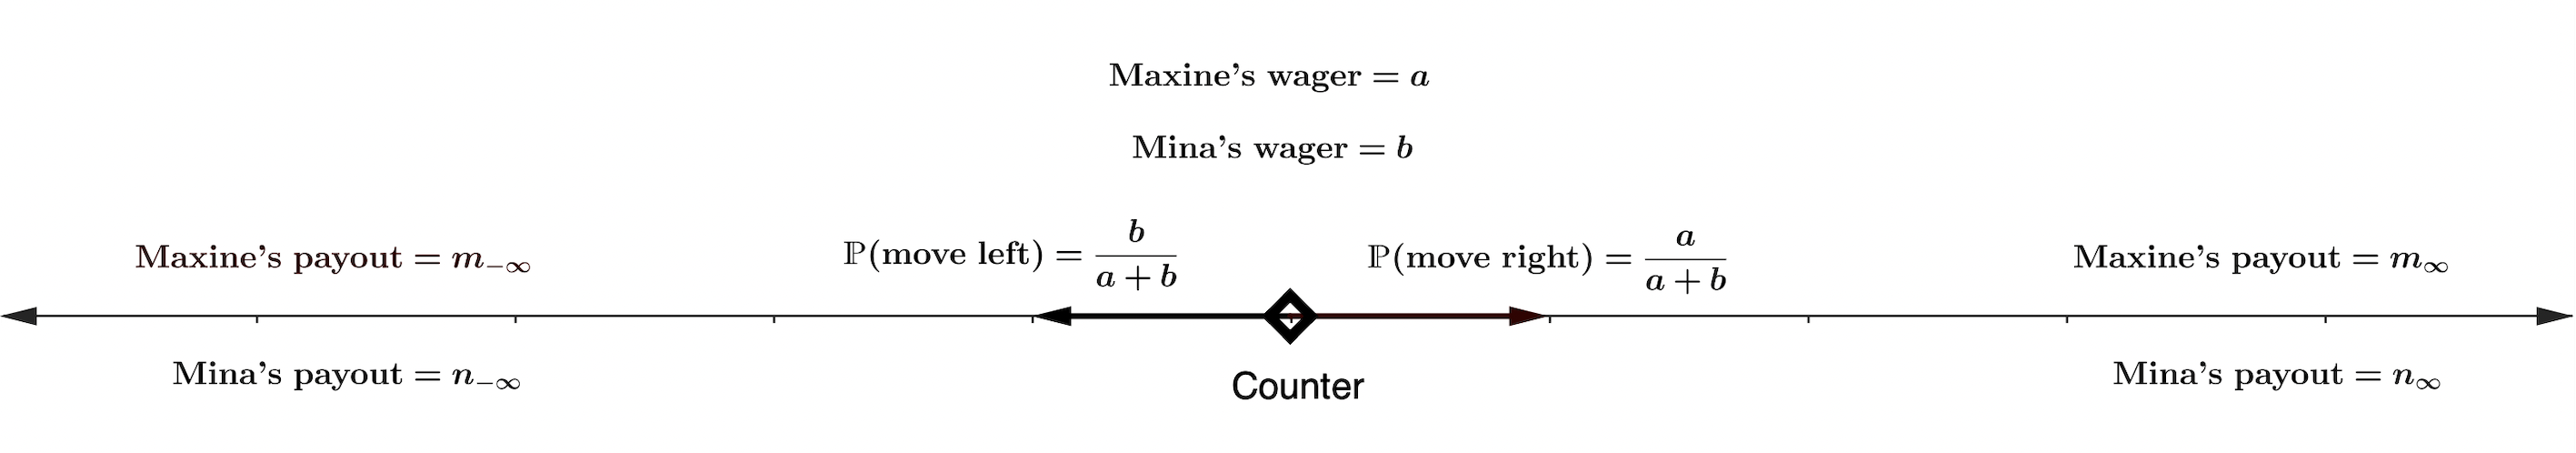
\includegraphics[scale=0.3]{infinite_trail.png}
    \caption{Trail($m_{-\infty}, m_{\infty}, n_{-\infty}, n_{\infty}$)}
\end{figure}

The infinite Trail game is very similar to the finite version, except that the game is played on the 
infinite integer line $\Z$ and the counter can move infinitely far to the left or right.

We denote the infinite Trail game as Trail($m_{-\infty}, m_{\infty}, n_{-\infty}, n_{\infty}$). The
game is set up such that $m_{-\infty}<m_{\infty}$ and $n_{\infty}<n_{-\infty}$, which ensures that
Maxine and Mina are always playing to the right and left respectively to maximize their payout.


\subsection{\centering Definitions (To be edited to keep only necessary and motivating definitions)}
The time-invariant Nash equilibrium of an instance of Trail($m_{-\infty}, m_{\infty}, n_{-\infty},
n_{\infty}$) are in fact characterized by the positive solutions to a system of equations, known as
the ABMN system, which we introduce here.

\begin{definition}[ABMN system]
    Let $a_i, b_i, m_i, n_i \in\R$ be the non-negative finite wager of Maxine and Mina, mean payout
    of Maxine and Mina respectively when counter is located at $i\in\mathbb{Z}$. Then the ABMN
    system is the set of equations 
    \begin{align}
        (a_i + b_i)(m_i + a_i) & = a_i m_{i+1} + b_i m_{i-1} \\
        (a_i + b_i)(n_i + b_i) & = a_i n_{i+1} + b_i n_{i-1} \\
        (a_i + b_i)^2 & = b_i (m_{i+1} - m_{i+1}) \\
        (a_i + b_i)^2 & = a_i (n_{i-1} - n_{n+1}),
    \end{align}
    where $i$ ranges over $\mathbb{Z}$. 
\end{definition}

\begin{definition}[ABMN solution]
    A solution to this system of equations is said to have boundary data $(m_{-\infty}, m_{\infty},
    n_{-\infty}, n_{\infty})$ when 
    $$\lim_{k\to\infty}m_{-k}=m_{-\infty}, \quad \lim_{k\to\infty}m_{k}=m_{\infty}, \quad
    \lim_{k\to\infty}n_{-k}=n_{-\infty}, \quad \lim_{k\to\infty}n_{k}=n_{\infty}.$$ For such a
    solution, the \underline{Mina margin} is set equal to
    $\frac{n_{-\infty}-n_{\infty}}{m_{\infty}-m_{-\infty}}$. A solution is called
    \underline{positive} if $a_i, b_i >0$ for all $i\in\mathbb{Z}$. It is called \underline{strict}
    if $m_{i+1}>m_i$ and $n_i>n_{i+1}$ for $i\in\mathbb{Z}$. (include strict ?)
\end{definition}

\begin{theorem}[Positive ABMN solution is time-invariant Nash equilibrium]
    Let $(m_{-\infty},m_{\infty},n_{\infty},n_{-\infty})\in\R^4$ satisfying $m_{-\infty}<m_\infty$
    and $n_\infty<n_{-\infty}$.
    \begin{enumerate}[label=(\arabic*)]
        \item Suppose that $\{(b_i, a_i):i\in\Z\}$ is a time-invariant strategy in the Nash
        equilibrium set. Then the quadruple $\{(a_i,b_i,m_i,n_i):i\in\Z\}$ is a positive ABMN
        solution boundary data $(m_{-\infty},m_{\infty},n_{\infty},n_{-\infty})$.
        \item Conversely, suppose that $\{(a_i,b_i,m_i,n_i)\in(0,\infty)^2\times\R^2:i\in\Z\}$ is a
        positive ABMN solution with boundary data $(m_{-\infty},m_{\infty},n_{\infty},n_{-\infty})$.
        Then $\{(b_i,a_i):i\in\Z\}$ is a time-invariant strategy in the Nash equilibrium set.
    \end{enumerate}
\end{theorem}

\begin{theorem}[Conditions for positive ABMN solution]
    Let $I\subset (0,\infty)$ equal to the set of values of the Mina margin
    $\frac{n_{-\infty}-n_{\infty}}{m_{\infty}-m_{-\infty}}$, where $\{(a_i, b_i, m_i,
    n_i)\in(0,\infty)^2\times \R^2:i\in\mathbb{Z}\}$ ranges over the set of positive ABMN solutions.
    Then,
    \begin{enumerate}[label=(\arabic*)]
        \item there exists a value $\lambda\in(0,1]$ such that $I = [\lambda, \lambda^{-1}]$;
        \item a positive ABMN solution exists with boundary data $(m_{-\infty}, m_{\infty},
        n_{-\infty}, n_{\infty})\in\R^4$ if and only if $m_{-\infty}<m_{\infty}$ and $n_{\infty} <
        n_{-\infty}$ and the Mina margin
        $\frac{n_{-\infty}-n_{\infty}}{m_{\infty}-m_{-\infty}}\in[\lambda, \lambda^{-1}]$;
        \item the value of $\lambda$ is at most 0.999904.
    \end{enumerate}
\end{theorem}

\section{\centering Proof}
\subsection{\centering Definitions}
\begin{definition}
    Set $w(x): (0,\infty)\to(1,\infty)=\sqrt{8x+1}$. Writing $w=w(x)$, we further set
    $$s(x)=\frac{(w-1)^2}{4(w+7)},\qquad c(x)=\frac{(w+3)^2}{16}, \qquad d(x)=\frac{(w+3)^2}{8(w+1)}
    \qquad \text{for } x\in(0,\infty).$$ For simplicity, we also write $s, c, d$ for $s(x), c(x),
    d(x)$ respectively.
\end{definition}

\begin{definition}
    Let $s_{-1}:(0,\infty)\to(0,\infty)$ be given by $s_{-1}(x)=\frac{1}{s(1/x)}$. Define
    \begin{enumerate}[label=(\arabic*)]
        \item $s_0 = x$.
        \item $s_i = \begin{cases}
            s(s_{i-1}), & i \geq 1 \\
            s_{-1}(s_{i+1}), & i \leq -1
        \end{cases}$.
        \item $c_i = c(s_i)$.
        \item $d_i = d(s_i)$.
    \end{enumerate}
\end{definition}

\begin{definition}
    Set $P_0=S_0=1$. For $k\in\N_+$, we specify 
    $$P_{k}(x)=\sum_{j=0}^{k-1}\left(\prod_{i=0}^{j}(c_i(x)-1)\right) + 1 \quad \text{and} \quad
    S_{k}(x) = \sum_{j=0}^{k-1}\left(\prod_{i=0}^{k}(d_i(x)-1)\right) + 1.$$

    Set $Q_1=T_1=0$. For $\ell\in\N_{\geq2}$, we then set 
    $$Q_{\ell}(x)=\sum_{j=1}^{\ell-1}\left(\prod_{i=1}^{j}(c_{-i}(x)-1)^{-1}\right) \quad \text{and} \quad
    T_{\ell}(x) = \sum_{j=1}^{\ell-1}\left(\prod_{i=1}^{k}(d_{-i}(x)-1)^{-1}\right).$$
\end{definition}

\begin{definition}[Finite-trail mina margin map]
    For $k\in\N$ and $\ell\in\N_+$, the finite mina margin map takes the form 
    $$\M_{\ell, k}(x)=\frac{x(S_k+T_\ell)}{P_k+Q_\ell}.$$
\end{definition}

\subsection{\centering Proof of conjecture}

\begin{lemma}
    There exists $x_0\in[\frac{1}{3},3]$ such that $\M(x_0)=\lambda$, and
    $$\lambda=\inf\{\M(x):x\in(0,\infty)\}.$$
\end{lemma}

\begin{lemma}
    For $x\in[\frac{1}{3}, 3], |\M(x)-\M_{5,4}(x)| \leq 6.3\times 10^{-7}$.
\end{lemma}

\begin{lemma}\indent
    \begin{enumerate}[label=(\arabic*)]
        \item $w, s:(0,\infty)\to(0,\infty)$ are increasing.
        \item $c, d:(0,\infty)\to(1,\infty)$ are increasing.
    \end{enumerate}
\end{lemma}

\begin{definition}
    For $[a, b]\subseteq (0,\infty)$, define 
    $$\M^\downarrow_{5,4}[a,b]=\frac{a(S_4(a)+T_5(b))}{P_4(b)+Q_5(a)}.$$
\end{definition}

\begin{lemma}
    For $[a,b]\subseteq(0,\infty)$, $\M^\downarrow_{5,4}[a,b]$ is a lower bound of $\{\M_{5,4}(x):
    x\in[a,b]\}$.
\end{lemma}
\begin{proof}
    Recall \emph{Lemma 3} and \emph{Definition 4}. By composing increasing function,
    $s_i, c_i, d_i$ are increasing functions for all $i\in\Z$. 
    
    Recall $P,S,Q,T$ from \emph{Definition 5}. By summing products of increasing, strictly positive
    functions, $P_k, S_k$ are increasing. By summing products of decreasing,
    strictly positive functions, $Q_\ell,T_\ell$ are decreasing.

    Therefore, for any $x$ in any interval $[a,b]\subseteq(0,\infty)$, 
    $$P_4(b) + Q_5(a) \geq P_4(x) + Q_5(x) \quad \text{and} \quad S_4(a)+T_5(b) \leq
    S_4(x)+T_5(x).$$
    
    Hence, $$\frac{a(S_4(a)+T_5(b))}{P_4(b)+Q_5(a)} \leq \inf\{\M_{5,4}(x):x\in[a,b]\}.$$
\end{proof}

\begin{theorem}[$\lambda \geq 0.999902$]
    Let $I=[\lambda,\lambda^{-1}]$ equal to the set of values of the Mina margin
    $\frac{n_{-\infty}-n_{\infty}}{m_{\infty}-m_{-\infty}}$, where $\{(a_i, b_i, m_i,
    n_i)\in(0,\infty)^2\times \R^2:i\in\mathbb{Z}\}$ ranges over the set of positive ABMN solutions.
    Then, the value of $\lambda$ is between 0.999902 and 0.999904.
\end{theorem}
\begin{proof}
    The upper bound has been proved in [Hammond].

    Following \emph{Lemma 1}, it suffices to show that
    $\lambda=\inf\{\M(x):x\in[\frac{1}{3},3]\}\geq0.999902$. Following \emph{Lemma 4}, it suffices
    to show that $\inf\{\M_{5,4}(x):x\in[\frac{1}{3},3]\}\geq 0.99990263$.

    By partitioning $[\frac{1}{3},3]$ into subintervals $\{t_0<t_1<\dots<t_n\}$, then 
    \begin{align*}
        \inf\{\M_{5,4}(x):x\in[\frac{1}{3},3]\} & =
        \min\{\inf\{M_{5,4}(x):x\in[t_{i-1},t_i]\}:i\in\{1,\dots,n\}\} \\
        & \geq \min\{\M^\downarrow_{5,4}[t_{i-1},t_i]:i\in\{1,\dots,n\}\}.
    \end{align*}
    A computer evaluation of the function with partition of mesh $=10^{-7}$ yields
    0.9999030108006773, which completes the proof. (Refer to the GitHub repository for the code.)
\end{proof}

\end{document}
